% !TeX spellcheck = en_US
\section{Results for the Degradations}
\label{sec:430_results_recording_degradations}
The results of the conducted subjective surveys are quality models for camera shake, harmful occlusions and camera misalignment, as shown in Table~\ref{tab:430_shaking}.
To generate the quality models, the ratings for each video sequence are gathered, normalized, and aggregated to ratings for all different characteristic combinations for all the three investigated degradations.
A model for each degradation is fitted by a linear regression on the normalized ratings for classified videos.
\begin{table}[!htb]
	\centering 
	\caption[Recording quality models]{Linear quality models for different video genres impaired by camera shake, harmful occlusions, and camera misalignment.}
	\resizebox{\columnwidth}{!}{\begin{tabular}{lccccccccccccc}
		\hline
		& \multicolumn{5}{l}{\textbf{Camera Shake}} & \multicolumn{4}{l}{\textbf{Harmful Occlusion}} & \multicolumn{4}{l}{\textbf{Camera Misalignment}} \\
		& \multicolumn{5}{c}{$a_0 + a_{ampl} * x_1 + a_{dur} * x_2 + a_{speed} * x_3  $} & \multicolumn{4}{c}{$b_0 + b_{size} * y_1 + b_{dur} * y_2 $} & \multicolumn{4}{c}{$c_0 + c_{perc} * z_1 + c_{dur} * z_2 $} \\ \hline
		Genre&  $a_{ampl}$ & $a_{dur}$ & $a_{speed}$ & $R^{2}$ & $MSE$ &  $b_{size}$ & $b_{dur}$& $R^{2}$ & $MSE$  & $c_{perc}$ & $c_{dur}$ & $R^{2}$ & $MSE$  \\ \hline
		Sports & -2.572 & -0.049 & -2.412 & 0.757 & 0.09 & -5.335 & -0.109 & 0.92 & 0.057 & -2.7 & -0.09 & 0.93 & 0.012\\
		Music & -0.873 & -0.068 & -2.961 & 0.742 & 0.089 & -4.35 & -0.09 & 0.77 & 0.168 & -1.82 & -0.04 & 0.62 & 0.18 \\
		Show  & -0.667 & -0.074 & -3.098 & 0.827 & 0.082 & -4.963 & -0.094 & 0.91 & 0.058 & -2.83 & -0.12 & 0.73 & 0.13 \\
		\hline
		
		\multicolumn{14}{l}{\textbf{Note:} Camera shake: $a_{ampl}$ - Amplitude [0-1], $a_{dur}$ - Duration [0-12 seconds],  $a_{speed}$ - Speed [0-1]} \\ 
		
		\multicolumn{14}{l}{Harmful occlusion: $b_{size}$ - Size [0-1], $b_{dur}$ - Duration [0-12 seconds]} \\ 
		\multicolumn{14}{l}{Camera misalignment: $c_{perc}$ - Percentage [0-1], $c_{dur}$ - Duration [0-12 seconds]}\\
		\hline
	\end{tabular} }
	\label{tab:430_shaking}
\end{table}
$R^2$ describes the coefficient of determination and is a metric to show the validity of the fitted model. Values close to $1$ are favored.
The proposed linear models achieve an $R^2$ of between 0.62 and 0.93, where solely the camera misalignment model for the music genre achieved an $R^2$ score of less than 0.73. 
$R^2$ predicts the variances in the quality assessments of our studies depending on the characteristics being assessed.
Thus, it depicts how well the proposed quality models describe the perceived quality for the different video genres. 

In the remaining section, these models are discussed in more detail.
An example of the influence of various degradations on a single video is given in Figure~\ref{fig:430_surface_degradation}.
\begin{figure}[htb]
	
	\centering
	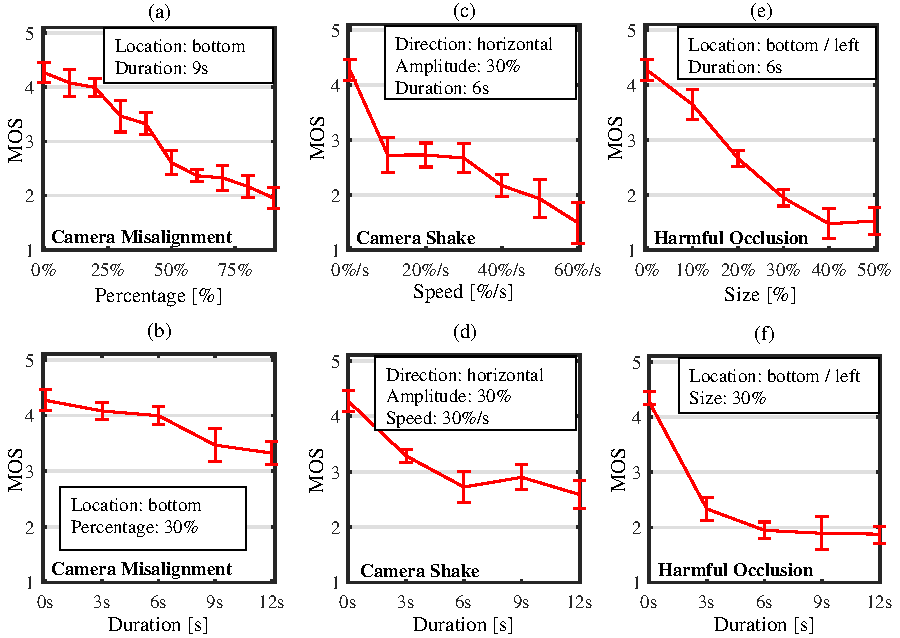
\includegraphics{gfx/400_UGV_Quality/degradationsSingle.pdf}
	\caption[Attributes of the perceived quality models for recording degradations]{MOS on perceived quality reduction due to Camera Misalignment (a)-(b), Camera Shake (c)-(d) and harmful occlusion (e)-(f). The upper row shows the reduction of the MOS depending on the intensity of the degradation whereas the bottom row shows the influence of the duration of a degradation (95\% confidence intervals - video: "PrincessRun").}
	\label{fig:430_surface_degradation}
\end{figure} 
\subsection{Camera Shakes}
\label{sec:430_results_camera_shakes}
Figure~\ref{fig:430_surface_degradation} depicts an example for the video sequence "PrincessRun", showing the relation of the speed of a shake $a_{speed}$ and its duration $a_{dur}$. 
In comparison with the harmful occlusions [(e)-(f)], it shows that the decrease in the perceived quality of short and slow camera shakes [(c)-(d)] is higher than the effect of a middle-sized harmful occlusion.
The characteristics investigated for camera shake include $a_{ampl}$ for the amplitude of the shake, $a_{dur}$ as the duration of the shake, and $a_{speed}$ as the speed of the degradation. 
Results clearly indicate that all the characteristics discussed have a significant negative impact on the perceived quality.
As a result, one can say that the presence of camera shake alone can reduce the perceived quality to a level not acceptable for viewers.
This means that with increasing amplitude, duration, and speed of the camera shake, the perceived quality decreases. 
The duration has only a small impact on the quality decrease.
This indicates that the pure existence of a slow camera shake over a longer time does not degrade the perceived quality in the same manner as a short but intensive shake.  

Even though the different characteristics cannot be easily mapped to one another, our results indicate that fast camera shakes quickly degrade the quality even more than other degradations.
\paragraph{Impact of the Genre}
Another observation is that a camera shake is perceived differently for different genres (see Table~\ref{tab:430_shaking}). 
Whereas "entertainment" and "music" sequences have similar characteristics, the amplitude of a shake in sports videos has a different effect on the perceived quality. 
The interpretation of this observation is that sports viewers are used to shaky recordings.
The duration of a camera shake has a slightly decreased impact in comparison with other genres.
The amplitude determines whether the \ac{RoI} is captured in the whole sequence.
A high amplitude means that during the shake the movement extends to a point where the \ac{RoI} is lost.
A severe decrease in perceived quality is observed in sports videos which usually focus on one distinct person, e.g., the leading ball player in soccer or a single driver in a motorbike race.
The increased amplitude leads to a loss of focus on the distinct person.

\paragraph{Direction of a Shake}
Another factor with only a small effect on the perceived quality is the distinction between horizontal shakes (uncontrolled panning) and vertical shakes (uncontrolled tilting). 

\begin{figure}[ht]
	\centering
	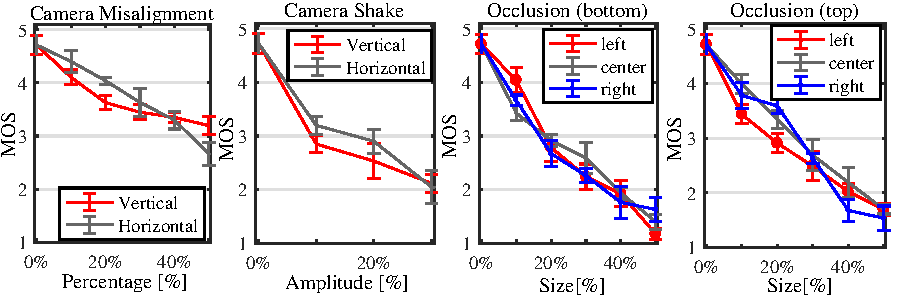
\includegraphics{gfx/400_UGV_Quality/location_relevance.pdf}
	\caption[Influence of the location where a degradation occurs on the perceived quality]{Influence of the location where a degradation occurs on the perceived quality for the video sequence "DanceKiss".
		The Figure includes the \ac{MOS} and the 95\% confidence intervals.}
	\label{fig:430_location_relevance}
\end{figure}
Figure~\ref{fig:430_location_relevance} illustrates that only in very few cases a difference between horizontal and vertical shakes for the sequence "DanceKiss" can be observed.
It can be concluded that camera shake algorithms can neglect to model the direction detection.
Similar findings are made for the other degradation types (see Figure~\ref{fig:430_location_relevance}).
As a result, the quality models proposed in Table~\ref{tab:430_shaking} neglect the direction as a characteristic.
\subsection{Harmful Occlusions}
\label{sec:430_results_occlusions}
An occlusion reduces the information a viewer can extract from a video sequence. 
Also, it is determined whether differences exist between different video genres. 
While evaluating harmful occlusions and their effect on the quality, the first attempt targeted occlusions at any position in the frame. 
Initial results show that spontaneously appearing objects at the border of the frame do not affect the quality at all.
This holds as long as the \ac{RoI} of a video frame is not affected. 
Only objects positioned in the line of sight between the camera and the \ac{RoI} are regarded as harmful.

Figure~\ref{fig:430_surface_degradation} (e)-(f) shows the reduction of quality depending on the size of the occlusion and the duration it is visible in a sequence. 
As mentioned, the size determines how much of the \ac{RoI} is occluded. 
The figure illustrates quite well that short, harmful occlusions or only small sizes of the occluding object reduce the quality by a limited amount.
Especially with increasing occlusion sizes, a rapid decrease in the quality can be observed. 
Occlusion sizes of 50\% result, independent of their duration, in a major reduction of the \ac{MOS} to values between 1 and 2. 
The observation is validated for the remaining video sequences. 
Table~\ref{tab:430_occlusion} shows the \ac{MOS} for increasing occlusion sizes of the occlusions for different video genres. 
For the selected video sequences, it shows a steady decrease of the quality for increasing sizes. 
\begin{table}[h]
\centering 
\begin{tabular}{cccc}
\toprule 
\backslashbox{Size}{Genre} & Sports & Music & Show\\ \midrule
0\% & 4.6  & 4.5 & 4.4 \\ 
10\% & 3.68  & 3.74 & 3.37 \\ 
20\% &  2.96 & 3.32 & 3.23   \\ 
30\% & 2.78  & 2.61 & 2.24  \\ 
40\% & 1.96 & 2.15 & 1.63  \\ 
50\% & 1.33 & 1.56 & 1.57  \\ 

\bottomrule
\end{tabular} 
\caption[MOS impaired by occlusions with varying size]{\ac{MOS} of different video genres impaired by harmful occlusions with varying size (duration: 6 seconds; position: bottom-center])}
\label{tab:430_occlusion}
\end{table}
The position of the occlusion has a limited impact on the perceived quality. 
Figure~\ref{fig:430_location_relevance} shows the difference for the sequence 
"DanceKiss" and for different locations at the bottom of the \ac{RoI}. 
Similar results are obtained from the top of the \ac{RoI} or any other region in the frame.
\subsection{Camera Misalignment}
\label{sec:430_results_misalignment}
The camera misalignment has only a limited impact on the perceived quality.
As the reference video is shown at least once during a task, it was easier for the workers to decide when a video sequence was recorded with a misaligned camera. 
Still, it is remarkable that especially the small pans or tilts of 10\% - 30\% result in a linear but limited decrease of the \ac{MOS}. 
In these cases, the perceived quality is still around 3.5, which indicates a still acceptable overall quality. %~\cite{???}. 
For the misalignment to degrade the perceived quality of a sequence to an undesirable level, the misalignment must affect the  \ac{RoI} of the video. 

Figure~\ref{fig:430_surface_degradation} (a-b) shows the resulting \ac{MOS} on the percentage of misalignment from the origin of the sequence "PrincessRun".
The figure supports this observation.
For the camera misalignment a decrease of the \ac{MOS} can be observed, but especially in the range of 10\% - 30\%, there is no significant reduction observable.
Additionally, Figure~\ref{fig:430_location_relevance} shows an investigation of the difference between the vertical and the horizontal misalignment.  
For the "DanceKiss" sequence, the quality degradation is higher for horizontal misalignments (at 40\%-50\%), i.e., a panning of the camera. 
The reduction of \ac{MOS} is observable especially in the range of 30\% - 50\%, and it results in a quality (\ac{MOS}) of around 1.5 for video sequences with up to 100\% misaligned recordings. 
\subsection{Existing Quality Algorithms}
As full reference metrics are not applicable, if a video is degraded during the recording, the analysis discusses the no reference video quality metric of Yang et al.~\cite{Yang2005} and the recently proposed \ac{V-BLIINDS} algorithm~\cite{Saad2014}.
Both metrics show reliable quality assessment in detecting compression effects.
They suffer in detecting the recording quality degradations discussed.
For the most severe degradation of camera shaking, Yang et al.~\cite{Yang2005} found a result of an average correlation of 0.31 across the genres.
Even \ac{V-BLIINDS}, which outperforms established full reference algorithms, achieves a correlation with subjective assessments on average of 0.608.
These findings illustrate a need for objective, \ac{NR} metrics measuring the impact of recording degradations and underlines the importance of this work.